% Ein Beispielkapitel
%

\chapter{Implementation}

The implementation which are done in this thesis enable to run the full mouse brain circuit.
Therefore a efficient data format is defined, the circuit generation scripts are adapted to
run on a bigger scale and the NEST simulator is extended to load the new data format.

\section{Data formats}
A point neuron circuit contains point neurons and connections (synapses) between the point neurons.
The same point neuron model and synapse model are used for all neurons and synapses respectively.
The neurons and synapses are characterized by parameters.
Each neuron is defined by a given set of parameters.
The synapses contain besides the parameters the source and target neuron id, which the synapses connects.
To store the circuit in files two different data formats are defined.
The first data format defines the storage for all neuron parameters.
The second data format defines the storage for the synapse parameters and source and target neuron ids.

The data format for the neurons and the synapses follow two different concepts.
The neuron data format contains multiple datasets containing the neuron parameters.
All datasets have by definition the same length. This length defines the number of neurons.
The neuron parameters of neuron $i$ are stored in the i-th line of each data set.
Besides the neuron parameters the file contains attributes for storing meta data of the circuit.
\begin{figure}[ht!]
   	\begin{center}
        \subfigure[HDF5 file format for the neurons]{%
            \label{fig:allInjections}
            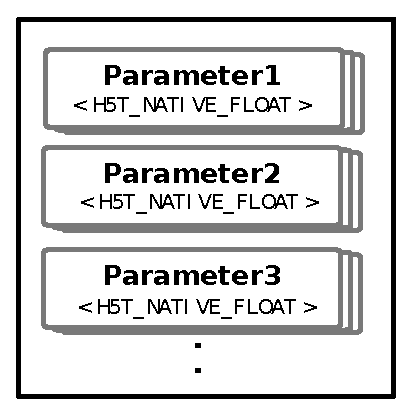
\includegraphics[scale=0.5]{pictures/hdf5_neuron_format.eps}
        }
        \hspace{1cm}
        \subfigure[HDF5 file format for the synapses]{%
            \label{fig:oneProjection}
            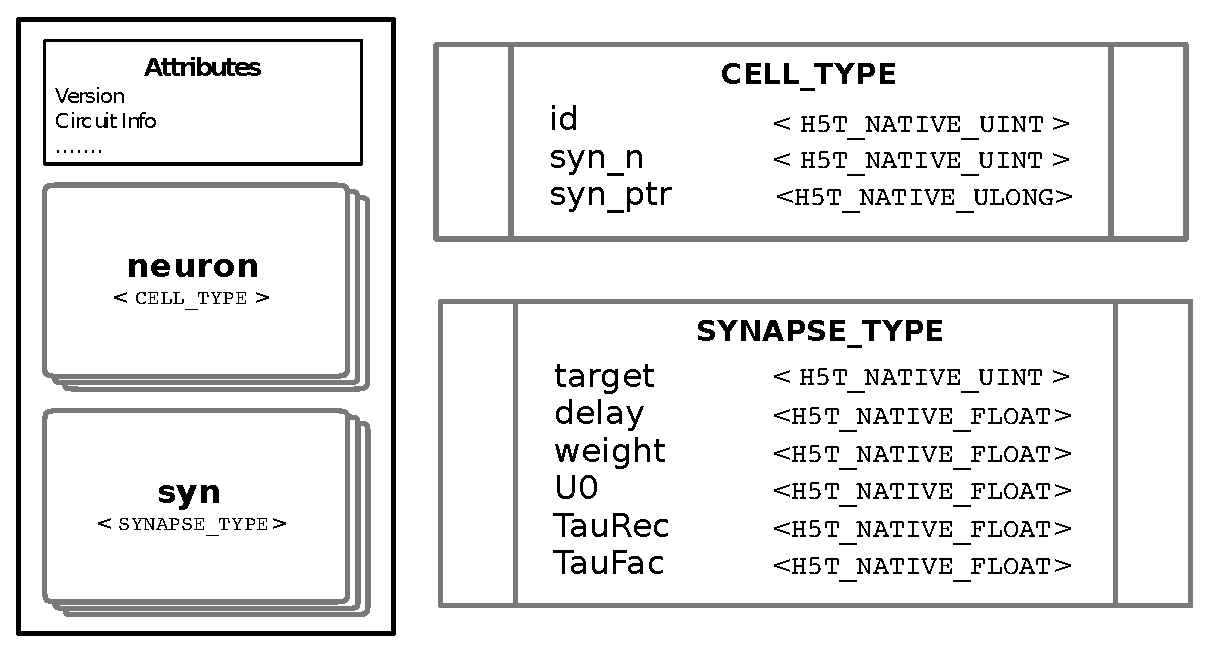
\includegraphics[scale=0.41]{pictures/hdf5_syn_format.eps}
       }
    	   \end{center}
    	\caption{%
        You can see the data format with their related datasets and data types. 
        How they are created by the circuit generation and loaded by the NEST import module.
     }%
   \label{fig:atlas}
   \end{figure}
The synapse data format contains only two datasets. In general the datasets contain for each synapse
a source neuron id, a target neuron id and a set of parameters. To reduce the amount of data.
The source neuron ids are grouped together in the \emph{neuron} dataset. This is feasible, because
the number of synapses is way bigger than the number of source neurons. The \emph{syn\_ptr} value 
defines the related starting index in the \emph{syn} dataset, respectively \emph{syn\_n} defines the
number of related following entries.
The \emph{syn} dataset contains the target neuron id and a set of parameters.
Both datasets use a compound data type to store different data types in the same dataset.

\newpage
\section{Circuit generation}
Rewriting the sequential python script to a hybrid C++ application require a parallel implementation of the algorithm and the usage of 
a parallel random generator. For the parallelization strategy a Master-Slave approach is chosen to distribute the workload dynamically on the nodes.
Communication between the individual nodes is not necessary. Only the workload management is handled by the master node.
For the random generator Random123 is used, because it has good performance and it is easy to use \cite{salmon2011parallel}.
It ensures reproducible results without correlations in the generated values, which is essential.


\subsection{Long range connections}

The long range generation algorithm is adapted so it can be parallelized.
The problem with the sequential algorithm is, that it iterates through all experiments
and generates all connections for all the voxels inside its injection regions, if 
all experiments before have not touched the voxels or have higher total injection
value. This means it generates connections which might be overwritten and each iteration might depend
on all previous iterations. To overcome this problem the best chosen injection is calculated before hand.
After that all voxels are distributed to the nodes and inside the iteration over all neurons
inside the given voxel, the sequential algorithm can be applied on each node.
Because the computation time needed by each voxel iteration varies a lot. Only the first third
of the voxels are distributed statically to the worker nodes.
All the other voxels are distributed dynamically by the master node.
The number of written entires can be calculated before hand. This allows to create
the HDF5 dataset before and assign a writing position to each voxel.
Thus all nodes can write independent to the file system.

\begin{itemize}
      \item parallelization strategy and implementation
      \item requirements 
\end{itemize}

\begin{figure}[ht!]
\centering
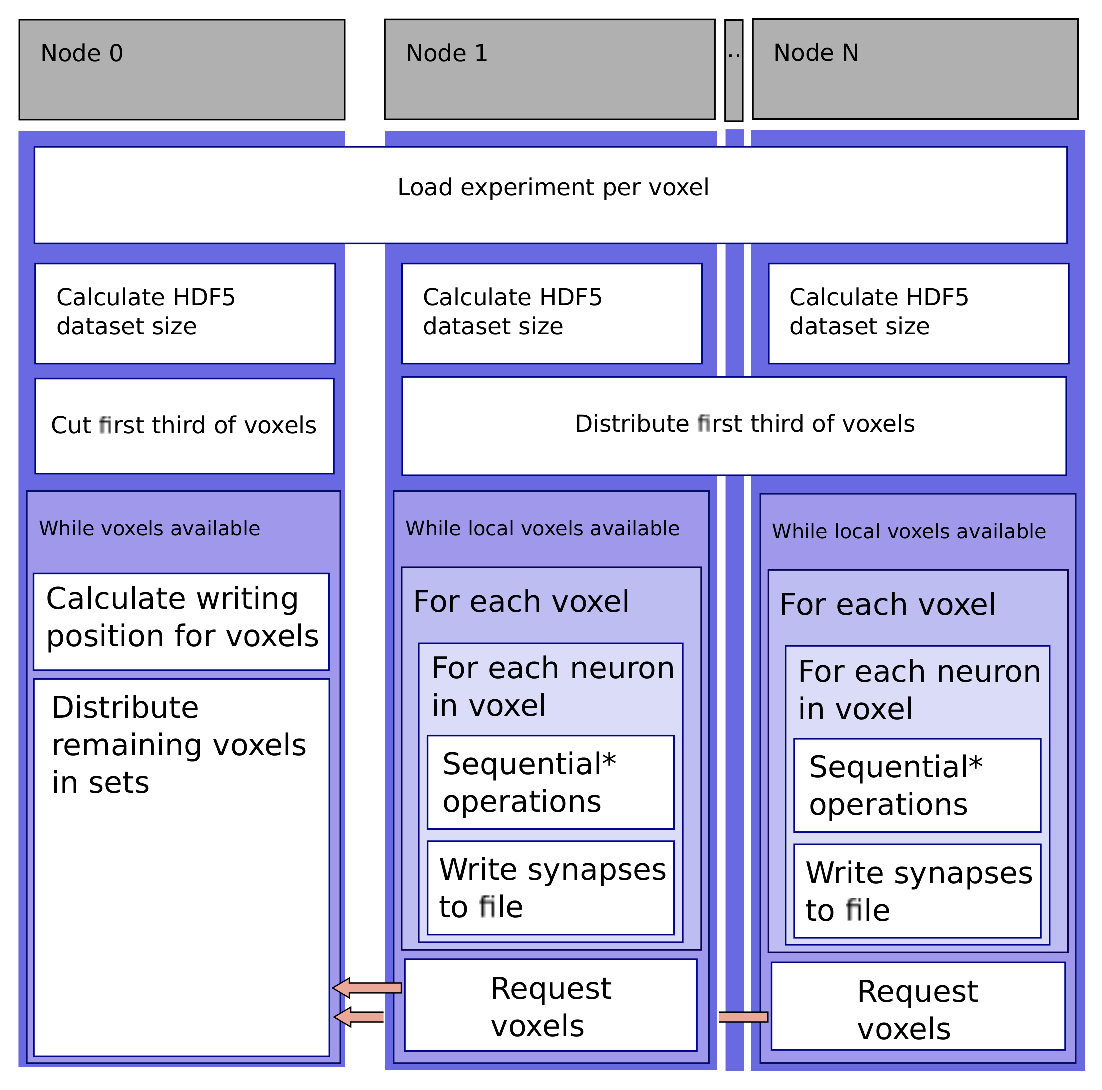
\includegraphics[scale=0.5]{pictures/longRange_parallelAlg.eps}
\caption{Task distribution between the nodes for the long range connections generation. It illustrates which tasks are distributed between which nodes.}
\end{figure}

\begin{figure}[ht!]
\centering
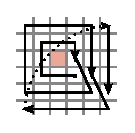
\includegraphics[scale=2.5]{pictures/longRange_Nearest_parallelAlg.eps}
\caption{Find nearest neighbor loop}
\label{longrange}
\end{figure}

The given algorithm was extended by a interpolation. There are voxels for which there is no injection of any experiment
available. To be able to generate connections for each neuron anyway. Voxels which are affected take the injection and projection from the nearest voxel with an injection. The strategy to find the nearest neighbor is an iteration around the neighborhood of each empty voxel. The Figure \ref{longrange} shows an illustration of the search algorithm
projected in a 2D plane. The first voxel along the search direction which is found is declared as ne nearest neighbor.


\begin{figure}[ht!]
\centering
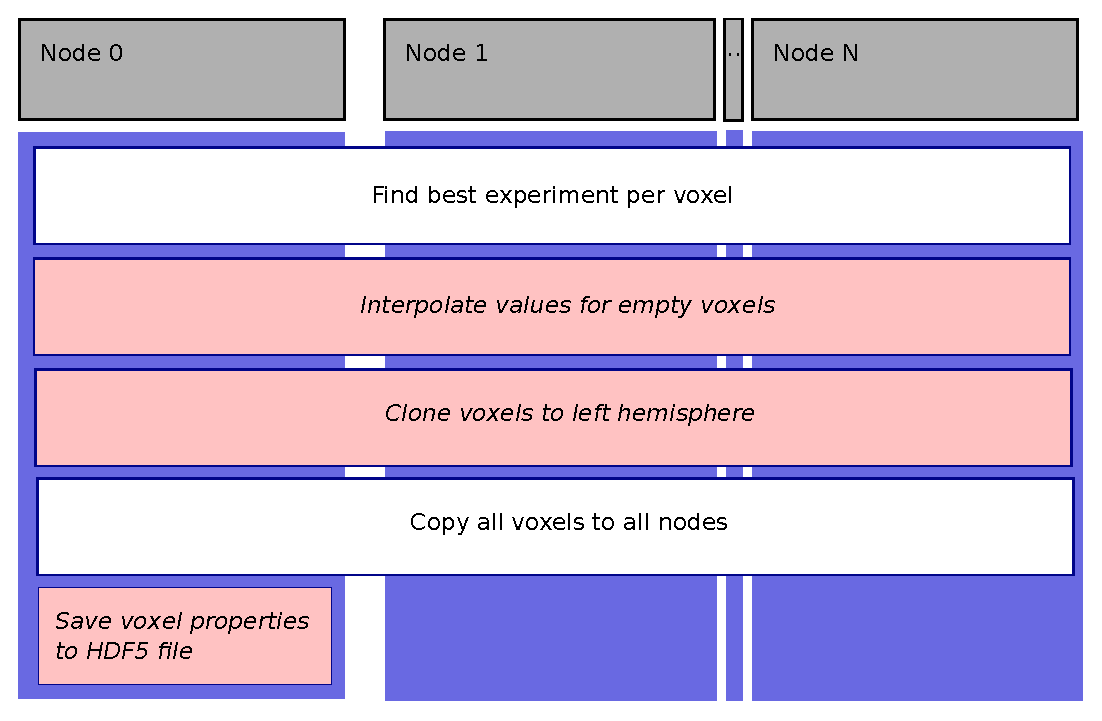
\includegraphics[scale=0.5]{pictures/longRange_BestExp_parallelAlg.eps}
\caption{Subtasks of the above listed \emph{Load experiment per voxel} task}
\end{figure}

\begin{figure}[ht!]
   	\begin{center}
        \subfigure[All nodes are equal and process the work based on a static distribution]{%
            \label{fig:shortColumn}
            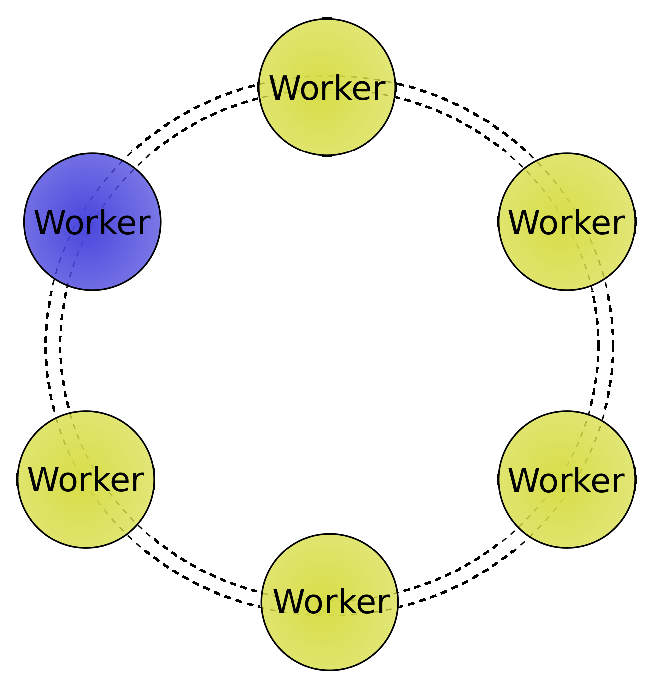
\includegraphics[scale=0.5]{pictures/All_Worker_Collective.eps}
        }
        \hspace{1cm}
        \subfigure[The 0 node is assigned as the master node and handles from this on the management of the work distribution.]{%
            \label{fig:shortColumnInCircuit}
            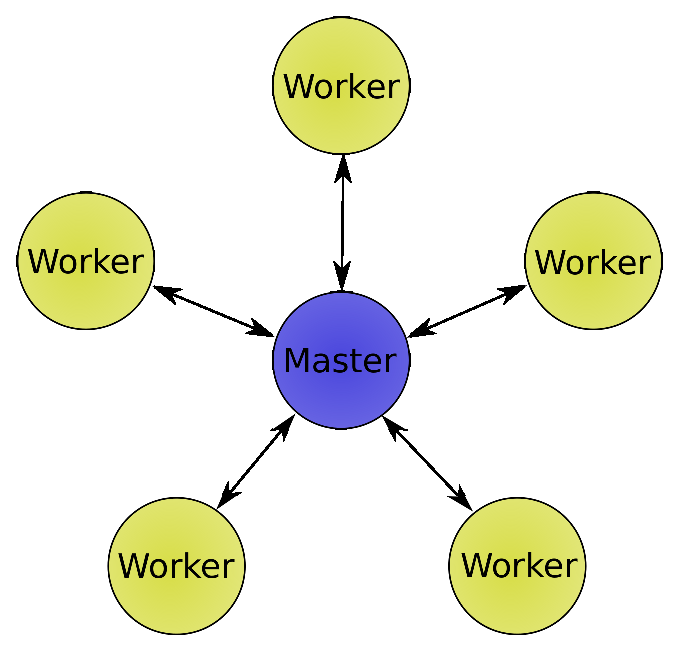
\includegraphics[scale=0.5]{pictures/MasterWorker.eps}
       }
    	   \end{center}
    	\caption{%
        The figure illustrates the work distribution and communication between the nodes.
     }%
   \label{fig:atlas}
   \end{figure}

\newpage
\subsection{Short range connections}

The algorithm presented in the analysis section can be parallelized straight forward.
Each iteration is independent. The challenging part is the distribution of the iterations and
the writing to disk. The number ob synapses which are created is not know. It is only available
at the end.

\begin{figure}[ht!]
\centering
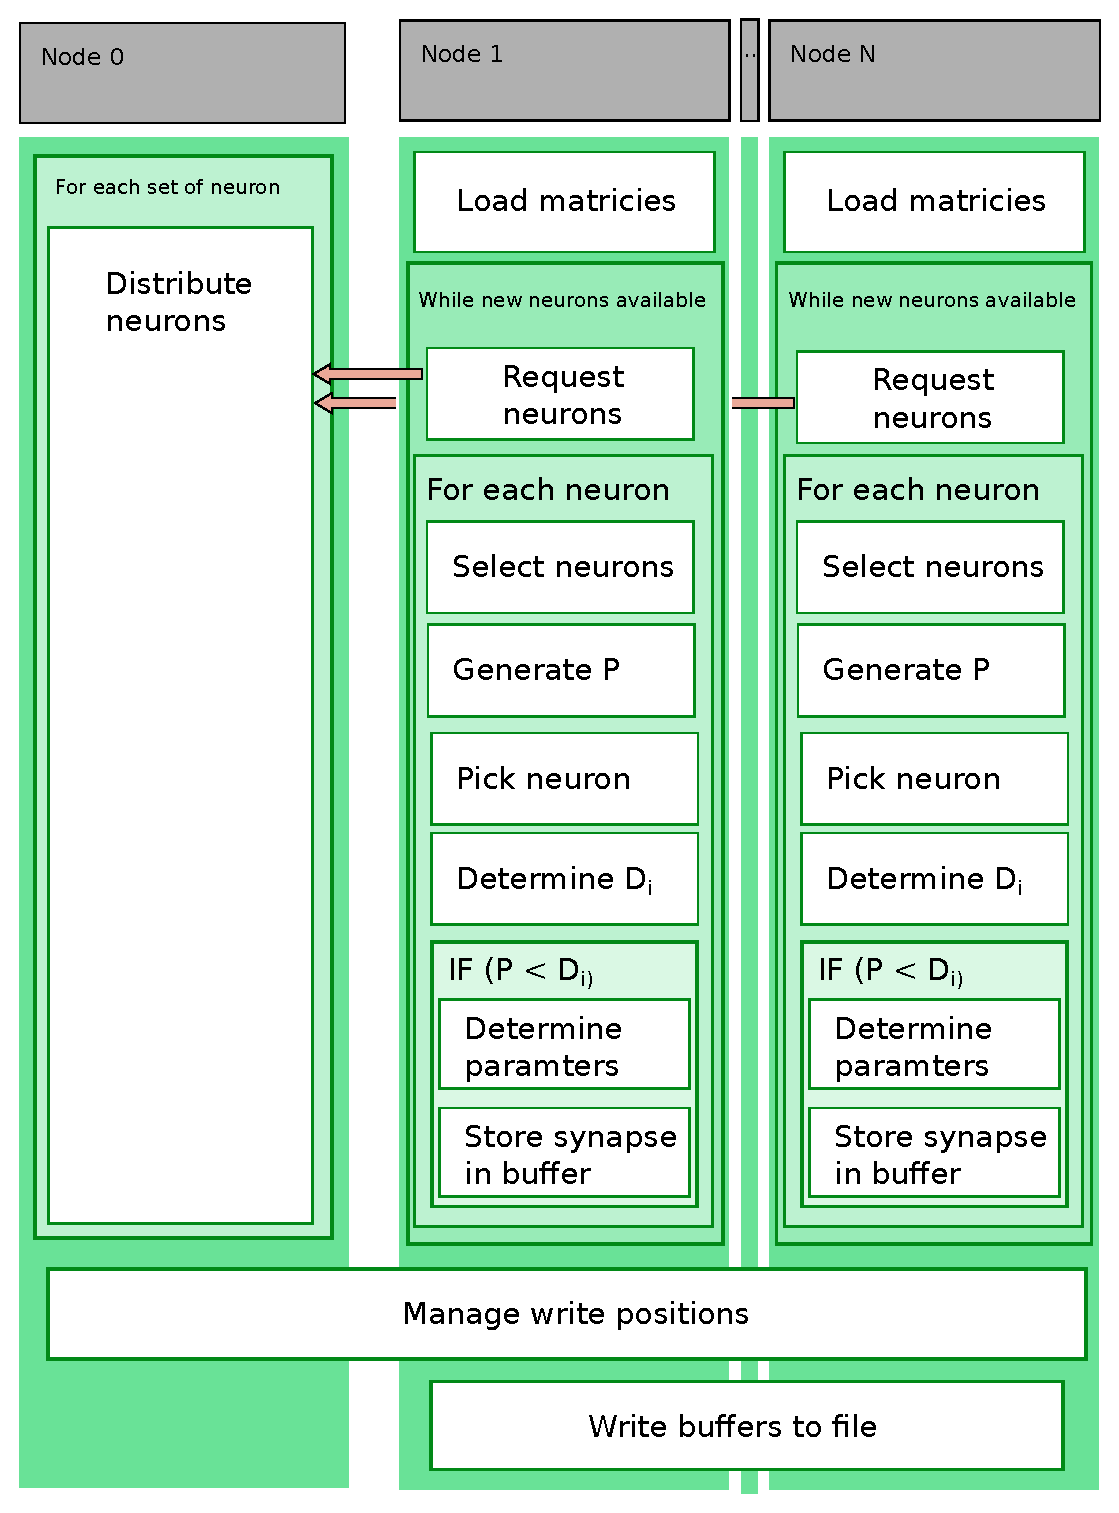
\includegraphics[scale=0.5]{pictures/shortRange_parallelAlg.eps}
\end{figure}

The short range algorithm is parallelized using a master-worker strategy to achieve a good load balancing.
The master node manages the distribution of the neurons, which can be seen as task units. For each neuron 
is synapses have to be created. The workers load in the first step all needed matrices from the file system.
Then each node request a set of neurons from the master node. Over this set it iterates and creates resulting
synapses. For \emph{Generate P} Random123 as a random number generator is used. Therefore a parallel usage of 
the given sequential algorithm is possible. Only the storage of the generated synapse list, has to be done 
after all iterations. So in each loop the synapse list is stored in a buffer.
If all neurons are distributed and processed all nodes, including the master node, calculate the position in 
the HDF5 dataset where each node is allowed to write. After that all workers write theirs synapse lists to
the HDF5 dataset.


\begin{figure}[ht!]
   	\begin{center}
        \subfigure[Master-worker strategy to get good balance properties]{%
            \label{fig:shortColumn}
            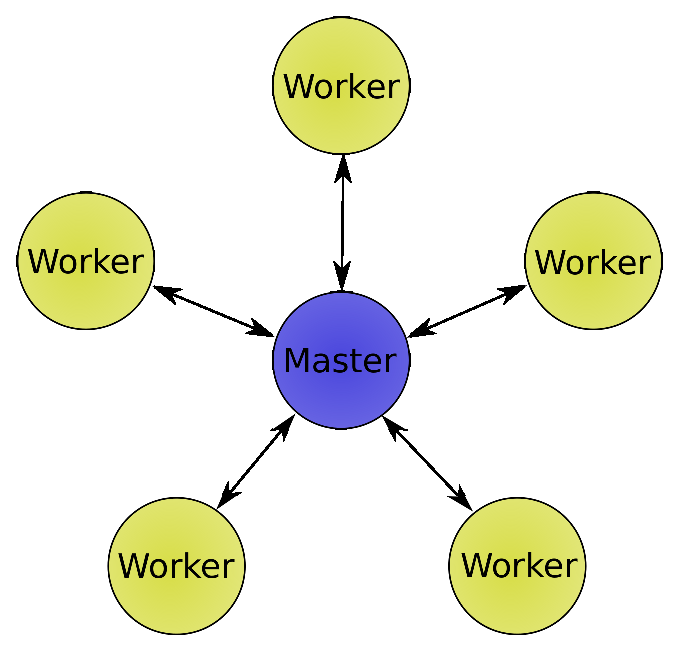
\includegraphics[scale=0.5]{pictures/MasterWorker.eps}
        }
        \hspace{1cm}
        \subfigure[Collective write operation to maximize used bandwidth]{%
            \label{fig:shortColumnInCircuit}
            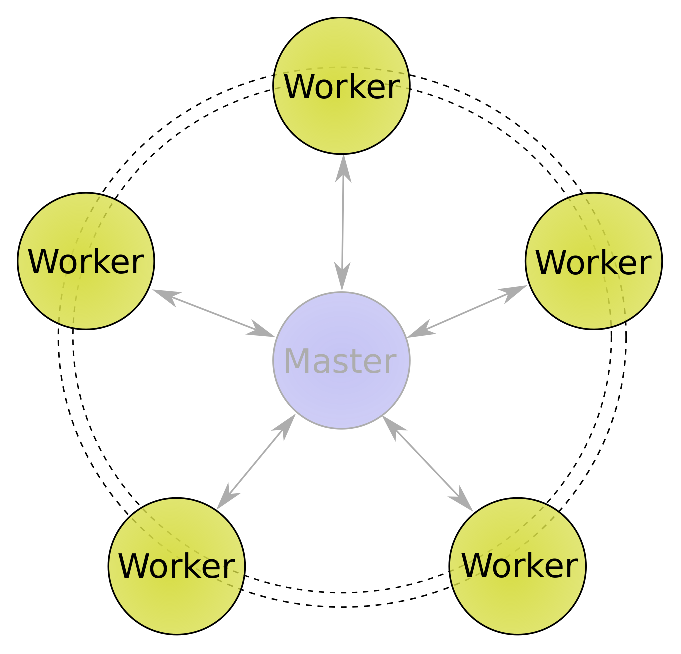
\includegraphics[scale=0.5]{pictures/Worker_Collective.eps}
       }
    	   \end{center}
    	\caption{%
        The figure illustrates the work distribution and communication between the nodes.
     }%
   \label{fig:atlas}
   \end{figure}
   
\begin{itemize}
      \item memory and computation requirements
\end{itemize}


\newpage
\section{Circuit validation}

In the context of this thesis the circuit is validated in terms of geometrical correct placement of
the synapses. So the position of the source and target can be visualized and be compared to a 
reference system. For the long and the short range connectivity the geometrical shape is know.
In particular the long range connectivity should connect neurons from the injected regions to neurons
in the projected region for each used experiment. Therefore a circuit for a single experiment is 
generated, the target and source neurons are visualized in a 3D coordinate system and the the injection
and projection is used as the reference system. If source neurons are inside the injection space and all
target neurons are in the projection space, the implementation is correct.
For the short range connectivity all post-synaptic neurons of synapses having the same pre-synaptic neuron should
lay inside a cylinder in layer 1 to 6. Visualising the post-synaptic neurons geometrical on top of the contour of layer 1 to 6 allows to review if the shape matches with a cylinder.
To perform the visual validation the renderer voxalize \ref{voxelize} is used with the visualization tool Paraview \ref{paraview}.
 \begin{figure}[ht!]
\centering
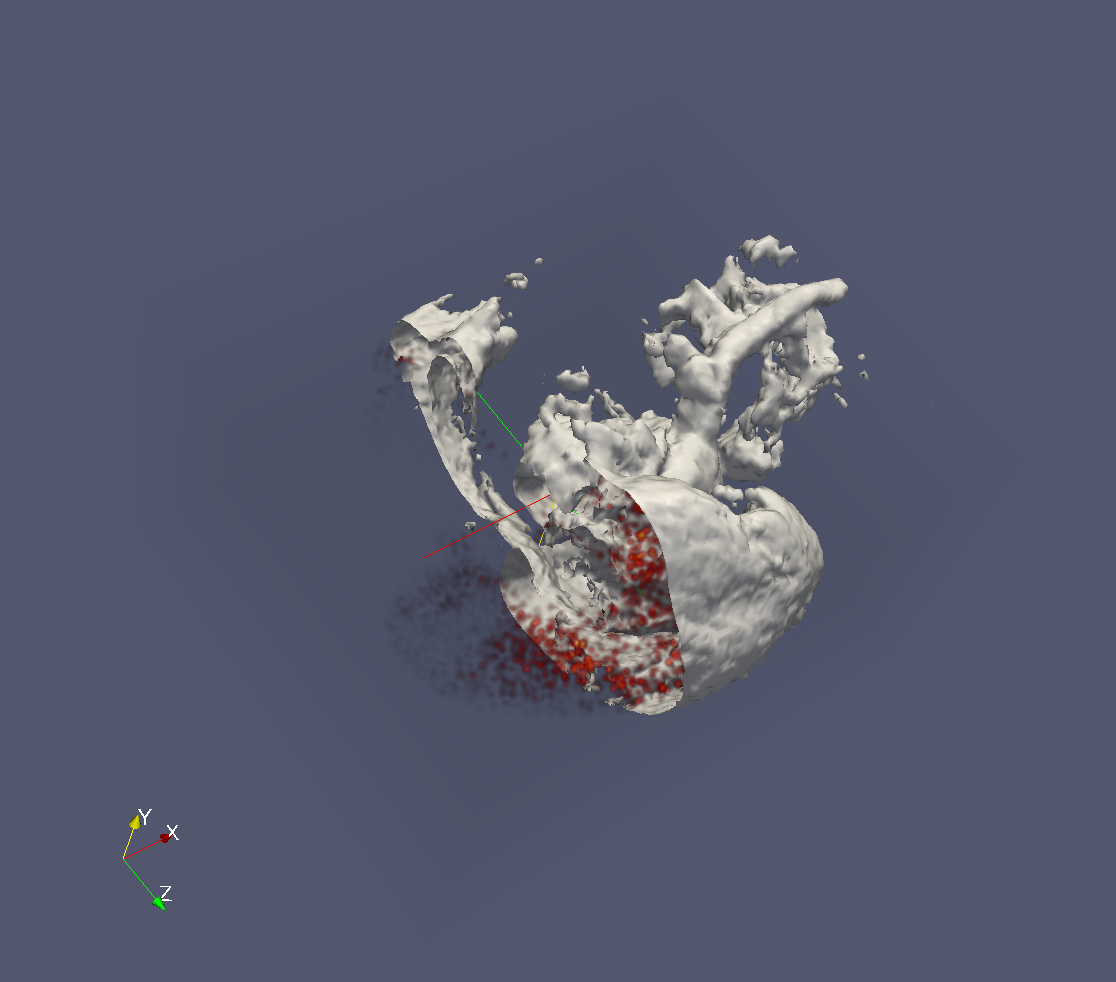
\includegraphics[width=0.4\textwidth]{pictures/paraview_ex.png}
\end{figure}
For the validation the BBP visualization team offered a rendering pipeline to visualize the placement of target neurons for each synapse file. Therefore the neuron and synapse HDF5 can be imported into 
Voxelize \ref{voxelize}. Voxelize creates a voxelized dataset out of the target neuron positions, which can be exported into
a MetaImage \ref{MetaImage} file or directly viewed with Livre \ref{Livre}.
The MetaImage files can be viewed with Paraview \ref{Paraview}.
Injection and projection images are also given in the MetaImage format.
A direct comparison inside of Paraview is possible.
Loading the projection inside of Paraview and applying the contour filter on it with a threshold of $0.01$ (threshold is also applied to the same data in the long range connectivity generation) allows to visualize the valid boundaries for all target neurons for this particular experiment.
 
\begin{itemize}
      \item Pictures of both validation
      \item Visual validation of spiking activity
      \item Statistical properties are not analyzed in this work 
\end{itemize}

\section{NEST import modules}
The neuronal spiking network simulator NEST is developed in \emph{C++} and delivers
an user interface based on an own description language \emph{SLI} and  and a Python interface.
The new use case shall be integrated into the standard work flow of NEST.
Besides the functionality in \emph{C++} the interfaces have to be extended.
The difficulties of the network generation is based on a difference in 
the NEST internal data structure and the data delivered by the Allen Institute.
Connection information contains target and source neurons besides biochemical
information of the synapses. Because of the in vitro injection methods the
connection information maps the synapse from the source to the target neurons.
For multi process simulations NEST distributes all neurons based on a modulo function 
to the processes. Because of memory optimizations the synapses are only stored on the
post synaptic process. This means that the connection information is stored
on the process, where the target neuron is located. Therefore a transformation of the given data is
necessary. Preprocessing of the input data should be avoided as far as possible to capture
future use cases.
The resulting implementation shall load the connection information efficiently in parallel,
distribute the synapse information to the post synaptic node and store it in
the NEST data structure.
Further requirements of the implementation are an efficient use of the available resources as
memory and computation power. 


\subsubsection{Import neurons}
To import neurons into NEST using the internal C++ API NEST has to create the requested number of neurons and
assign their parameters afterwards. In an distributed environment the create function has to be called on all nodes. But assigning the parameters has only be done on the nodes, where the neurons are placed on.
Thus only a set of the parameter datasets is needed on each node.
To group neurons together to subnets, neurons can be created inside of virtual subnets.
This subnets have to be created before hand.
\begin{algorithm}
 \KwData{HDF5 neuron dataset}
 \KwResult{Created neurons inside NEST data structure}
 Find unique values in subnet dataset; \\
 Create subnet for each unique entry; \\
 Create neurons based on length of HDF5 datasets with given neuron type inside specified subnets; \\
 Read parameter datasets collectively; \\
 Assign parameters to neurons;
\label{alg2}
\caption{}
\end{algorithm}
Therefore the implemented algorithm sorts out the needed subnets in its first step.
Unique values are extracted from the subnet dataset.
After that for each unique value a subnet is created.
In the next step the neurons are iteratively created inside the specified subnet.
Then the parameter values are loaded from the HDF5 datasets and committed to the neurons.
The neurons are stored distributed on the nodes.
So the neuron parameters are only needed on the node, where the neuron is placed.
The distribution is known. NEST distributes the neurons based on the modulo of their ids. Neuron $i$ is placed on node $i mod number\_of\_nodes$. Each node has to load all needed parameter entries
from the datasets. Derived from the distribution function each node has to load each number\_of\_nodesths entry starting from its node id.

\newpage
\subsubsection{Import synapses}
Synapse import module reads the the synapse dataset block wise. Using hyperslabs each node selects a block from the
dataset and copy it to memory with all the specified parameters.
The source neuron list and the target neurons and their parameters from each block are used to create a list of all synapses.
For each entry the target node is determined.
The list is sorted by the target nodes.
Using \emph{MPI\_Alltoall} the list can be distributed directly to the corresponding nodes.
Afterwards each node contains its list of synapses and can use the \emph{NEST} connect function, to copy it to its internal data structure.
\begin{algorithm}
	\KwData{List of HDF5 files for each node, chunk size}
	\KwResult{Connected NEST network}
	\While{Chunk to read in HDF5 files}{
		Read block and store in memory \hspace{45px}(1)\;
 Determine target node for each synapse \hspace{63px}(1,2) \hspace{36px}$\mathcal{O}(n)$\;
 Sort synapses by target nodes \hspace{66px}(1,2) \hspace{28px}$\mathcal{O}(n^2)$\;
 MPI\_Alltoallv using sorted list \hspace{76px}(1,2,3,4)\;
 Connect all synapses using NEST function \hspace{36px}(1,2) \hspace{45px}$\mathcal{O}(n)$\;
	}
\label{alg2}
\caption{Distribute connection information without transposing, $S_i$ source neuron $i$, $Tn_i$ target neuron $i$.
	set in brackets contains current needed variables}
\end{algorithm}



\begin{figure}[ht!]
\centering
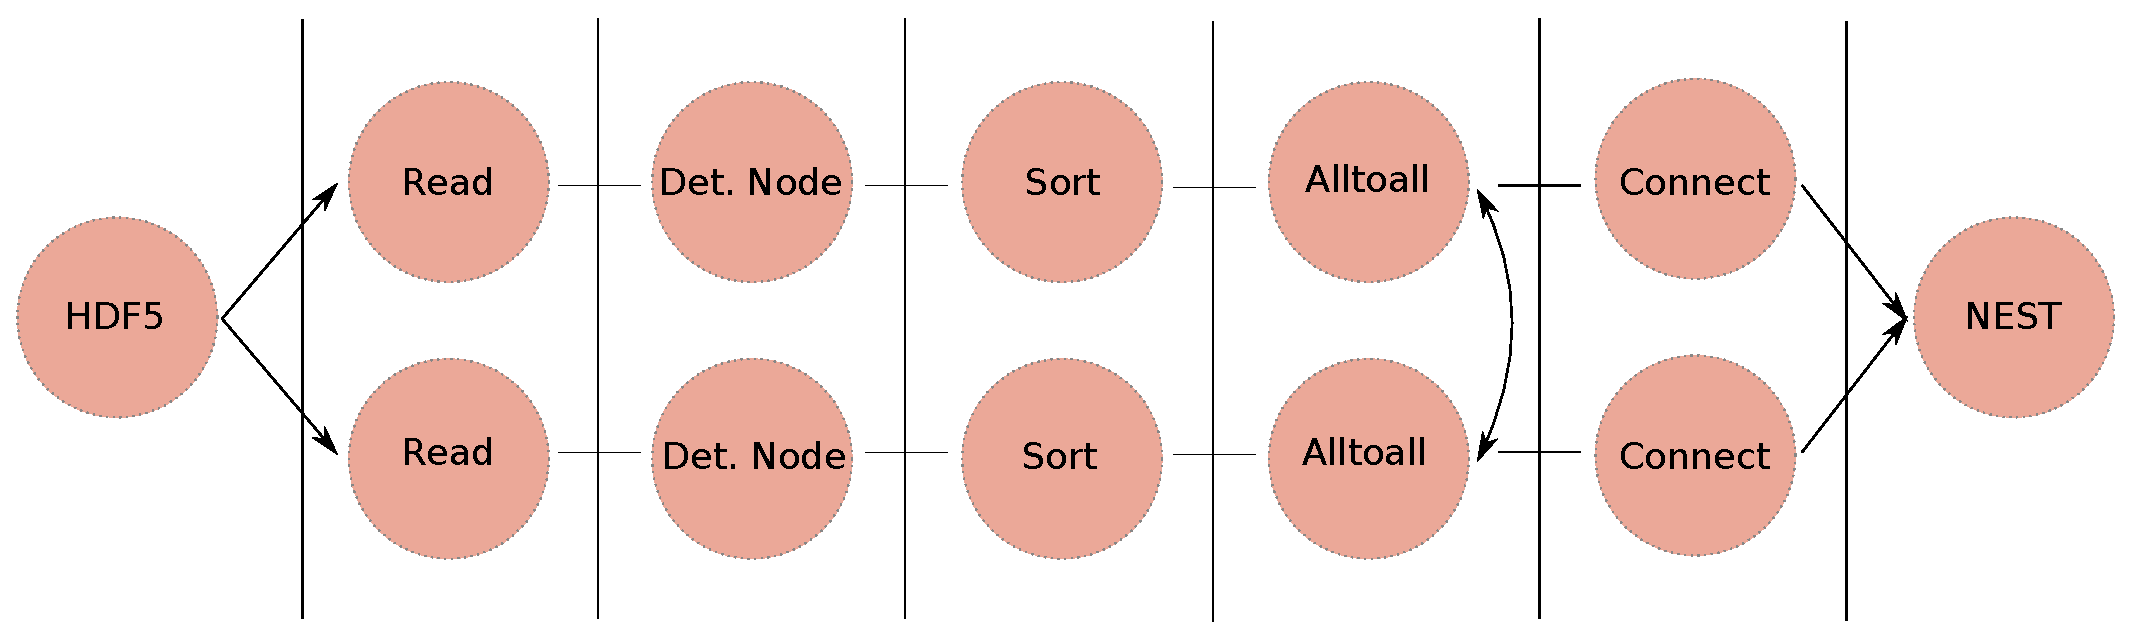
\includegraphics[scale=0.4]{pictures/Connect_inside_iteration.eps}
\caption{Inside iteration parallel workflow}
\end{figure}

\begin{figure}[ht!]
\centering
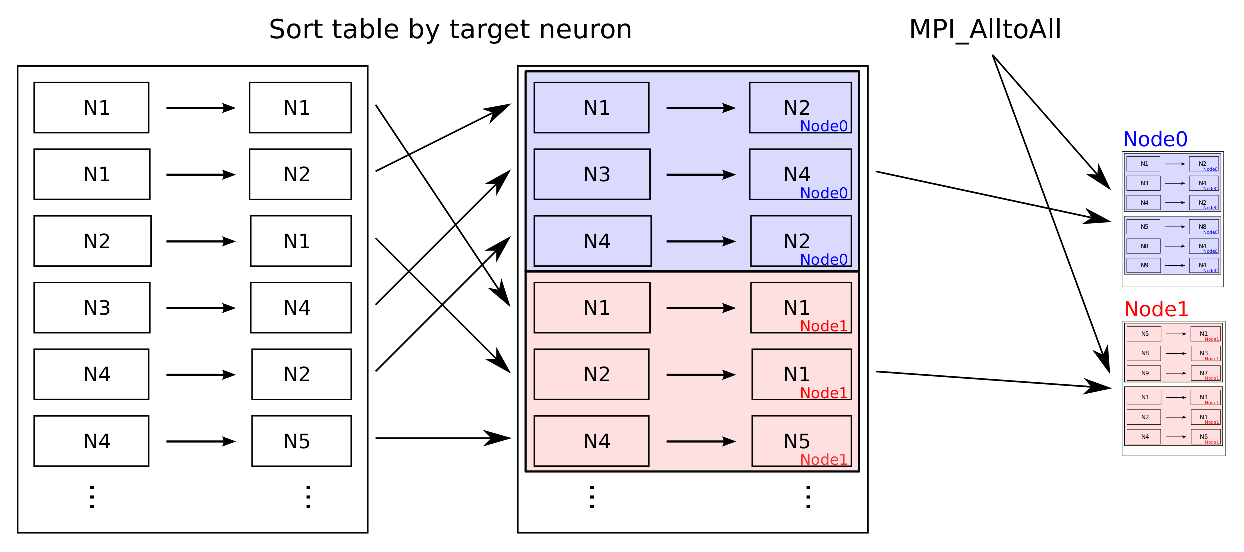
\includegraphics[scale=0.7]{pictures/sort_table_all_alltoall.eps}
\caption{Distribute synapses to the nodes.}
\end{figure}


\lstdefinestyle{cppcode} {language=C++,
                basicstyle=\tiny\ttfamily,
                keywordstyle=\color{blue}\ttfamily,
                stringstyle=\color{red}\ttfamily,
                commentstyle=\color{green}\ttfamily,
                morecomment=[l][\color{magenta}]{\#}
                numbers=left,
  				stepnumber=5,    
  				firstnumber=1,
 				numberfirstline=true
}
\begin{figure}[ht!]
\begin{lstlisting}[style=cppcode]
    void H5Synapses::singleConnect(NESTNodeSynapse& synapse,
    	nest::index synmodel_id,
    	nest::Node* const target_node,
    	const nest::thread target_thread,
    	uint64_t& n_conSynapses)
{
  nest::index source = synapse.source_neuron_;
  
  // check whether the target is on this process
  if (nest::NestModule::get_network().is_local_node(target_node)) {
    // use region to allow setting lock for creating/destroying token
    {     
      DictionaryDatum d( new Dictionary );
      
      //new/delete Token is not thread-safe
      omp_set_lock(&tokenLock);
      for (int i=0; i<synapses_.prop_names.size(); i++)
	def< double_t >( d, synapses_.prop_names[i], synapses_.prop_facts[i] * synapse.prop_values_ [i] + param_offset[i]);
      omp_unset_lock(&tokenLock);

      bool success = nest::NestModule::get_network().connect(source, target_node->get_gid(), d, synmodel_id);
 
      if (success)
	n_conSynapses++;
      
      omp_set_lock(&tokenLock);
    }
    omp_unset_lock(&tokenLock);
  }
  else
  {
    throw nest::IllegalConnection("H5Synapses::singleConnect(): synapse is on wrong node");
  }
}
\end{lstlisting}
\caption{Code copied from the import module, showing the used NEST c++ api. Appropriate size seems hard to find }
\end{figure}

\begin{itemize}
      \item describe use of NEST c++ api, lock has to be used
\end{itemize}

\newpage
\section{Memory consumption}
\begin{figure}[ht!]
\begin{tabular}{| l | l | l | l |}
    \hline
    (id) & data structures & memory consumption \\ \hline
    (1) & block in memory & $sizeof(float)*h*p$ \\ \hline
    (2) & target neuron node list & $sizeof(int)*h$ \\ \hline
    (3) & MPI send vectors & $(sizeof(float)*p + sizeof(int)) * h$ \\ \hline
    (4) & MPI recv vectors & $(sizeof(float)*p + sizeof(int)) * \frac{h}{\nu(N)}$ \\ \hline
    \end{tabular}
\caption{$N$: number of nodes; $h$: size of block; $p$: number of parameters; $\nu(N)$: distribution coefficient of data}
\end{figure}
The maximum memory consumption is:
\begin{equation}
  M = (sizeof(float)*p + sizeof(int)) * 2h * (1 + \frac{1}{\nu(N)})
  \label{eq:maxmemoryconsumption}
\end{equation}